\subsection{CajaMar Models}
\label{Section:CajaMarModels}

\subsubsection{Introduction}

There are two tasks to be solved for Cajamar's use case (see D1.2 and DoW). The main one is
the estimation of the \emph{probability of default}, defined as the probability that a
credit operation will end up to a default in two years. The other task is to obtain 
good customers profiles in terms of risk so that marketing campaigns can be
specifically directed to low risk customers. 

%%%%%%%%%%%%%%%%%%%%%%%%%%%%%%%%%%%%
\subsubsection{Predicting probability of default}
%%%%%%%%%%%%%%%%%%%%%%%%%%%%%%%%%%%%

%---------------------------------------------------------------------------------------------

The main task is predicting the probability that an operation will result in a default
\textbf{2 years before} it actually happens. It is therefore a \emph{supervised classification} problem,
currently solved using \emph{logistic regression} over \emph{27 predictors}. These predictor variables (many  of them manually built by CajaMar's experts) 
describes the financial behaviour of the customers in the last 180 days, which is a limit imposed by the Bank of Spain.  
The provided database is \emph{imbalanced} -around 10\% of defaulters-. 

We will initially consider two different approaches.

\subsubsection*{Static Model} 

In this first approach we ignore the dynamics of the problem: we do not model that a customer can be non-defaulter and defaulter at different moments in time (e.g. one customer can be creditworthy and, after some time, be in bankrupt for becoming unemployed). Here we just build a prediction model where given the financial behaviour of the client over the last 180 days, it predicts whether the client will default or not in 2 years. 

Figure \ref{Figure:CajaMarStatic} shows the general structure of this static model. Each yellow box represents a set of variables measures during the same day.
The variables within a box can be connected (e.g. according to a tree structure and, globally, conforming a TAN). The model only considers variables referring to the last 180 days. The red node models the possibility that the customer is a defaulter in the next two years. 

The process of building this static model would consist of the following steps:


\begin{itemize}
\item Construct a single flat table, containing information on time windows of \emph{180 days}.
\item Build a BN classifier (i.e. NB or TAN). 
\item Update risk profiles using the classifier.
\end{itemize}

\begin{figure}[ht]
\begin{center}
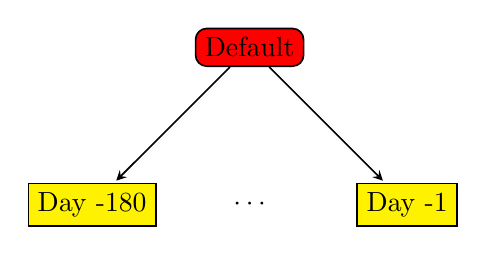
\begin{tikzpicture}[->,>=stealth,shorten >=1pt,auto,node distance=2cm,semithick,
        amarillo/.style={fill=yellow,rectangle,draw},
        rojo/.style={fill=red,rectangle,draw,rounded corners}]
        \node[rojo] (default) {Default};
        \node (dot) [below of=default] {$\cdots$};
        \node[amarillo] (tran1) [left of=dot] {Day -180};
        \node[amarillo] (tran180) [right of=dot] {Day -1};
        \draw (default) to (tran1);
        \draw (default) to (tran180);
\end{tikzpicture}
\end{center}
\caption{\label{Figure:CajaMarStatic}Global structure of the static model. Each yellow box represents a set of variables measures during the same day.
The variables within a box can be connected (according to a tree structure and, globally, conforming a TAN).}
\label{fig:static}
\end{figure}
%---------------------------------------------------------------------------------------------


\begin{figure}[ht]
\begin{center}
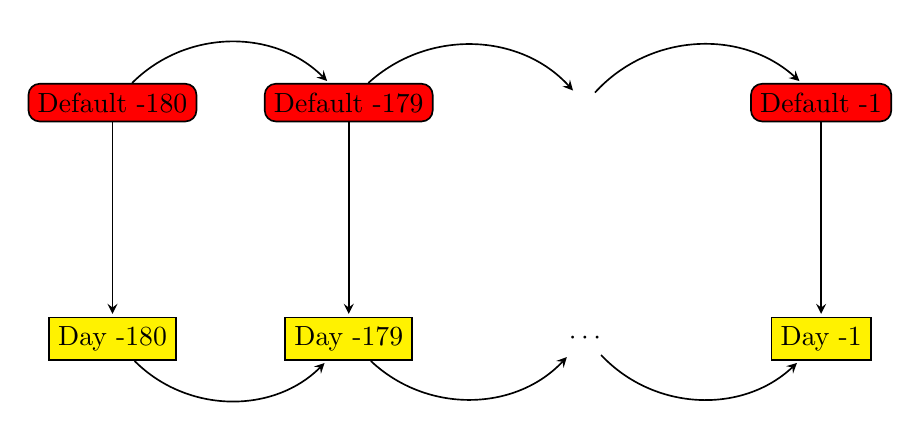
\begin{tikzpicture}[->,>=stealth,shorten >=1pt,auto,node distance=3cm,semithick,
        amarillo/.style={fill=yellow,rectangle,draw},
        rojo/.style={fill=red,rectangle,draw,rounded corners}]
        \node[rojo] (default1) {Default -180};
        \node[amarillo] (tran1) [below of=default1] {Day -180};
        \node[rojo] (default2) [right of=default1] {Default -179};
        \node[amarillo] (tran2) [below of=default2] {Day -179};
        \node (dot) [right of=tran2] {$\cdots$};
        \node (blank) [above of=dot] {$~~$};
        \node[amarillo] (tran180) [right of=dot] {Day -1};
        \node[rojo] (default180) [above of=tran180] {Default -1};
        \draw (default1) to (tran1);
        \draw (default2) to (tran2);
        \draw (default180) to (tran180);
        \draw (default1) to [bend left=45] (default2);
        \draw (default2) to [bend left=45] (blank);
        \draw (blank) to [bend left=45] (default180);
        \draw (tran1) to [bend right=45] (tran2);
        \draw (tran2) to [bend right=45] (dot);
        \draw (dot) to [bend right=45] (tran180);
\end{tikzpicture}
\end{center}
\caption{Global structure of the dynamic model. Each yellow box represents a set of variables measures during the same day.
The variables within a box can be connected (according to a tree structure and, globally, conforming a TAN) as well as variables between two consecutive days. Red box refer to the possibility that 
client is defaulter and are temporal connected.}
\label{fig:global_temp}
\end{figure}
%---------------------------------------------------------------------------------------------


%---------------------------------------------------------------------------------------------
\subsubsection*{Dynamic Model} 

In this approach we will consider the the dynamic structure of the problem. These dynamics are present because the behaviour of the customers evolves over time (e.g. the account balance is continuously changing from month to another, the level of incomes, etc.)  as well as the labelling as defaulter or non-defaulter customer (e.g. one customer can be creditworthy and, but after some time, be in bankrupt for becoming unemployed). 


\begin{figure}[ht]
\begin{center}
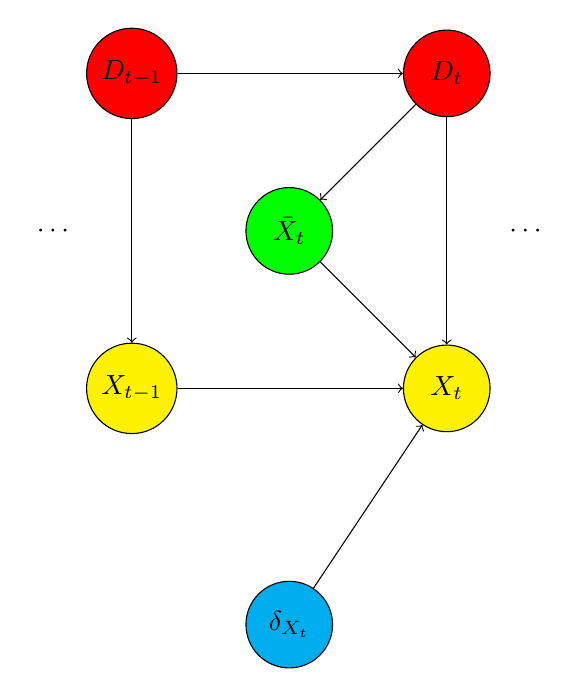
\begin{tikzpicture}
  \node[circle,fill=yellow,draw, minimum size=1.1cm] (Xt1) at (1,1) {$X_{t-1}$};
  \node[circle,fill=yellow,draw, minimum size=1.1cm] (Xt) at (5,1) {$X_t$};
  \node[circle,fill=green,draw, minimum size=1.1cm] (avg) at (3,3) {$\bar{X}_t$};
  \node[circle,fill=cyan,draw, minimum size=1.1cm] (ind) at (3,-2) {$\delta_{X_t}$};
  \node[circle,fill=red,draw, minimum size=1.1cm] (D) at (5,5) {$D_t$};
  \node[circle,fill=red,draw, minimum size=1.1cm] (Dt1) at (1,5) {$D_{t-1}$};
  
  \node at (0,3) {$\cdots$};
  \node at (6,3) {$\cdots$};
  
  \draw[->] (Dt1) to (Xt1);
  \draw[->] (Dt1) to (D);
  \draw[->] (D) to (Xt);
  \draw[->] (D) to (avg);
  \draw[->] (Xt1) to (Xt);
  \draw[->] (avg) to (Xt);
  \draw[->] (ind) to (Xt);
  
  
  
\end{tikzpicture}
\end{center}
\caption{Basic component of the structure of the dynamic model.}
\label{fig:component}
\end{figure}

Figure~\ref{fig:global_temp} represents the global idea of the temporal model. It can be compactly
represented by a dynamic Bayesian network made of components as the one displayed in 
Figure~\ref{fig:component}. $D_t$ represents the class variable at time slice $t$ (i.e. defaulting or non-defaulting client). Each feature
variable at time $t$, denoted as $X_t$, is linked to the same variable at time $t_1$: $X_{t-1}$
as well as to a \emph{memory variable} $\bar{X}_t$ that represents the average value of $X$
during the last $180$ time slices (days). Finally, an indicator variable $\delta_{X_t}$ may
be included if the variable is such that is observed many times at point 0. This is the case as,
for instance, payments by credit card, where many of the days can be equal to zero for most of
the customers.


The process of building this static model would consist of the following steps:

\begin{itemize}
\item Construct \emph{1 table} for each day.
\item Build a \emph{dynamic} BN classifier (NB or TAN like structure extended in a dynamic fashion). 
\item Update risk profiles using the classifier.
\end{itemize}





%\subsubsection*{Model Structure}
%
%From a probabilistic modelling point of view, Caja-Mar faces two different problems [][]: the prediction of the risk of defaulting of a customer in the next two years; and the extraction of profiles of ``desirable'' prospective customers. 
%
%The risk prediction problem has been modelled as supervised dynamic prediction problem.  We are given a data base with a set of variables or predictors (some of them manually built by CajaMar's experts) describing the financial behaviour of the customers and, also, whether the customer is considered as defaulter and non defaulter according to CajaMar standards (i.e. a binary class variable). The dynamic component of the problem needs to be considered because the behaviour of the customers evolves over time (e.g. the account balance is continuously changing from month to another, the level of incomes, etc.)  as well as the labelling as defaulter or non-defaulter customer (e.g. one customer can be creditworthy and, but after some time, be in bankrupt for becoming unemployed). More specifically, the proposed model is expected to answer the following question: which is the probability that this customer will  default in some of his/her loans in two years? And this prediction has to be made only using the customer's behavior in the last 180 days \footnote{This limit is imposed by the Bank of Spain.}.
%
%The graphical structure of the dynamic probabilistic graphical model devised for this problem is given in Figure \ref{Figure:CajaMarModel1}.  The yellow square boxes ``Day -180'', ..., ``Day-1'' represents the temporal evolution of the predictor variables. The model only refers to 180 days because this is the imposed limit of days when making predictions. Similarly, the class variable ``default'' is assumed to evolve over time but with the relevant different that the default class sequence refers to a point in the time \textbf{two years later} than  the point in the time the daily predictor variables. 



\subsubsection*{Data Analysis}

